\documentclass{beamer}
 
\usepackage[utf8]{inputenc}
 
%Information to be included in the title page:
\title{Linear Regression}
\subtitle{\small Research Methods}
\author{{\small Alex Hamelink \and Jos van Goor \and Bart Louwers}}
\institute{
    University of Groningen\\
    Faculty of Mathematics and Natural Sciences
}
\date{11 January 2016}
 
\begin{document}
 
\frame{\titlepage}
 
\begin{frame}
\frametitle{What is linear regression?}
\end{frame}

\begin{frame}
\frametitle{Assumptions}
\begin{enumerate}
\item \textbf{Linearity} between the dependent and independent variables.
\item \textbf{Homoscedasticity}.
\item \textbf{Normality} of the error distribution.
\end{enumerate}

We can test the assumptions by looking at plots generated by the plot.lm function.
\end{frame}

\begin{frame}
\frametitle{Assumptions}
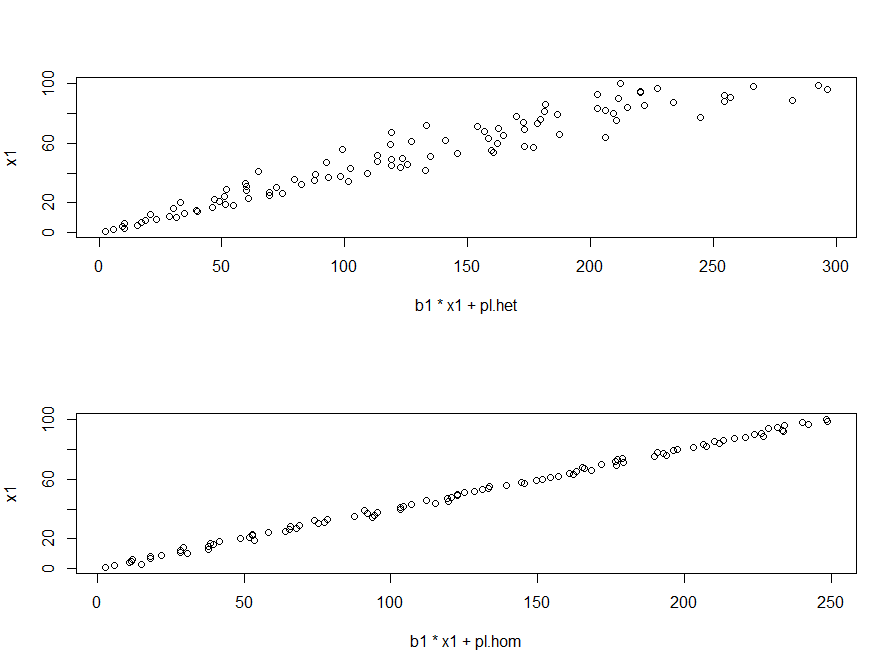
\includegraphics[width=\linewidth,height=\textheight,keepaspectratio=true]{hetvshom.png}
\end{frame}

\begin{frame}
\frametitle{Assumptions}
\begin{enumerate}
\item \textbf{Linearity} between the dependent and independent variables.
\item \textbf{Homoscedasticity}.
\item \textbf{Normality} of the error distribution.
\end{enumerate}

We can test the assumptions by looking at plots generated by the plot.lm function.
\end{frame}

\begin{frame}
\frametitle{Assumptions}
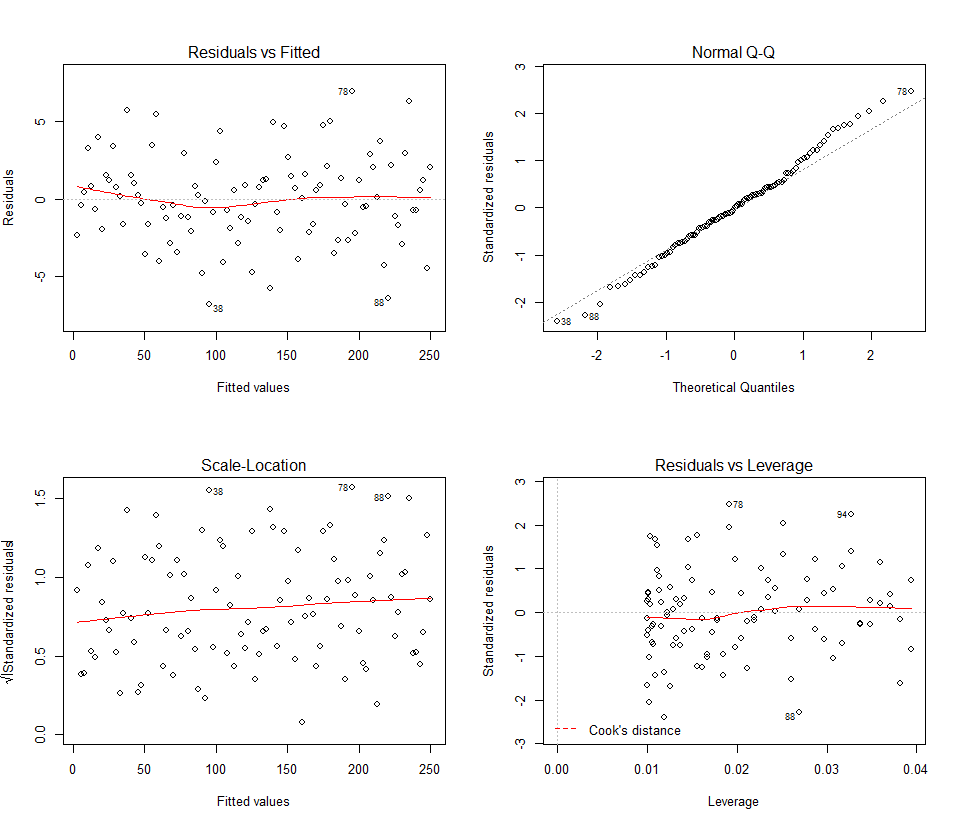
\includegraphics[width=\linewidth,height=\textheight,keepaspectratio=true]{lmplot.png}
\end{frame}
 
\end{document}
